% ============================================================================
% Beyond In-Domain Accuracy: Cross-Dataset Generalization and Deployment
% Analysis of Object Detectors for Autonomous Driving
%
% Modular LaTeX paper assembled from docs/final_paper/sections/*.tex.
% Tables are generated from validated project artifacts by
%   scripts/final_paper/generate_tables.py
% and figures by
%   scripts/final_paper/generate_figures.py
% See docs/final_paper/README.md for compilation instructions.
% ============================================================================

\documentclass[10pt,a4paper]{article}

\usepackage[T1]{fontenc}
\usepackage[utf8]{inputenc}
\usepackage{lmodern}
\usepackage{amsmath,amssymb}
\usepackage{graphicx}
\usepackage{booktabs}
\usepackage{caption}
\usepackage{microtype}
\usepackage[a4paper,margin=1in]{geometry}

% Hyperlinks and cross-references
\usepackage[colorlinks=true,linkcolor=blue,citecolor=blue,urlcolor=blue]{hyperref}

% Keywords command (IEEE-style index terms under the abstract)
\providecommand{\keywords}[1]{%
  \par\vspace{0.6em}\noindent\textbf{Index Terms---} #1\par}

\title{Beyond In-Domain Accuracy: Cross-Dataset Generalization and Deployment
Analysis of Object Detectors for Autonomous Driving}

% NOTE: replace with the actual author list and affiliation.
\author{Author Name}
\date{}

\begin{document}

\maketitle

% Abstract
\begin{abstract}
Reliable object detection is essential for autonomous-driving perception, yet most
detectors are evaluated primarily on data drawn from the same benchmark used for model
development. Such in-domain evaluation may overestimate deployment reliability when
geographic context, camera characteristics, scene density, object scale, and annotation
policies change. This study presents a controlled cross-dataset evaluation of four
representative detection paradigms: a YOLO-family real-time one-stage detector, Faster
R-CNN, RetinaNet, and RT-DETR. All models are trained on harmonized KITTI data and
evaluated first on a held-out KITTI validation split and then on a representative Waymo
front-camera subset without retraining, fine-tuning, or target-domain adaptation. Vehicle,
Pedestrian, and Cyclist categories are aligned across datasets to support consistent
comparison. The evaluation combines mAP, precision, recall, F1-score, per-class AP,
absolute and relative performance degradation, and a generalization ratio, together with
safety-oriented analyses of false negatives, small and occluded objects, and vulnerable
road users. Deployment suitability is assessed using batch-one latency, throughput,
parameter count, and model size on common hardware. The results show a severe and
architecture-dependent accuracy drop under target-free transfer: mAP@$[0.50{:}0.95]$
falls from $0.538$--$0.690$ on KITTI to $0.065$--$0.097$ on Waymo, with generalization
ratios between $0.095$ and $0.180$. The in-domain ranking inverts across domains:
YOLOv8s is strongest in-domain but least stable, while RetinaNet is weaker in-domain yet
most stable out-of-domain. On the external dataset, small objects and vulnerable road
users are the dominant failure mode, with pedestrian-plus-cyclist false-negative rates of
$0.81$--$0.93$ even for the most accurate detector. By unifying external validation,
safety-relevant failure analysis, and efficiency measurement, the proposed framework
determines whether strong in-domain accuracy translates into robust and practical
intelligent-vehicle perception.
\end{abstract}

\keywords{cross-dataset generalization, object detection, autonomous driving, domain shift,
deployment analysis, vulnerable road users.}

% Introduction
\section{Introduction}
\label{sec:introduction}

Modern object detectors achieve strong results on autonomous-driving benchmarks, but
these results are typically reported under in-domain evaluation, in which the training and
test data are drawn from the same dataset distribution. This setting can hide sensitivity
to dataset bias and may not reflect how reliably a detector behaves when deployed in a
different environment~\cite{geiger2012kitti,sun2020waymo}. In practice, a perception
system trained in one city or on one sensor configuration must operate in scenes with
different camera characteristics, traffic density, object-scale distributions, and
annotation conventions, and it remains unclear whether a high in-domain score translates
into robust performance under such shift.

This uncertainty is particularly important for safety-critical classes such as pedestrians
and cyclists, and for small, distant, occluded, and crowded objects. A detector that
attains a strong aggregate mean Average Precision (mAP) may still miss a large fraction
of vulnerable road users after a domain shift, an effect that aggregate metrics conceal.
Deployment constraints introduce a further dimension: a highly accurate detector may be
impractical at the required frame rate, while a very fast detector may be insufficiently
reliable for safety-critical perception~\cite{yang2022streaming,wang2023asap}. A
unified assessment of accuracy, external generalization, safety-oriented failure, and
computational efficiency is therefore needed to identify a defensible
accuracy--generalization--efficiency trade-off.

This study investigates the external generalization of object detectors trained on the
KITTI dataset~\cite{geiger2012kitti} and evaluated, without retraining, fine-tuning, or
target-domain adaptation, on a representative front-camera subset of the Waymo Open
Dataset~\cite{sun2020waymo}. Four detector families spanning representative detection
paradigms are considered: YOLOv8s (real-time one-stage CNN),
Faster R-CNN~\cite{ren2015fasterrcnn} (two-stage region proposal),
RetinaNet~\cite{lin2017focalloss} (dense one-stage with focal loss), and
RT-DETR~\cite{zhao2024rtdetr} (real-time transformer). All models are trained on the
same harmonized three-class task (Vehicle, Pedestrian, and Cyclist) under a common
experimental protocol, and evaluated in-domain on KITTI and externally on Waymo with a
frozen operating point. The evaluation combines in-domain accuracy, absolute and relative
cross-dataset degradation, a generalization ratio, class-wise behavior, safety-oriented
failure analysis, and same-hardware efficiency measurement.

The main contributions of this work are:

\begin{enumerate}
    \item \textbf{Controlled cross-family comparison.} A harmonized benchmark is
    developed for four representative detection paradigms under identical data,
    class, and evaluation rules.
    \item \textbf{Target-free external validation.} Models trained exclusively on
    KITTI are evaluated directly on Waymo with no retraining, fine-tuning, domain
    adaptation, or target-dependent selection.
    \item \textbf{Dataset and class harmonization.} A transparent class-mapping
    procedure aligns KITTI and Waymo annotations into the common Vehicle, Pedestrian,
    and Cyclist classes (Section~\ref{sec:datasets}).
    \item \textbf{Cross-dataset generalization analysis.} Generalization is quantified
    using in-domain and external mAP, absolute and relative degradation, a
    generalization ratio, and class-wise AP changes
    (Section~\ref{sec:results}).
    \item \textbf{Safety-oriented failure analysis.} False negatives, vulnerable road
    users, small and distant objects, and error types are examined alongside aggregate
    accuracy (Section~\ref{sec:results}).
    \item \textbf{Deployment-oriented efficiency evaluation.} Latency, throughput,
    parameter count, and model size are reported on common hardware
    (Section~\ref{sec:results}).
\end{enumerate}

The remainder of this paper is organized as follows. Section~\ref{sec:related_work}
reviews related work, Section~\ref{sec:datasets} describes dataset preparation and class
harmonization, Section~\ref{sec:methodology} details the preprocessing and validation
pipeline, Section~\ref{sec:experimental_setup} presents the training and evaluation
protocol, Section~\ref{sec:results} reports the results, Section~\ref{sec:discussion}
discusses their implications, Section~\ref{sec:threats} describes threats to validity,
and Section~\ref{sec:conclusion} concludes.

% Related Work
\section{Related Work}
\label{sec:related_work}

\subsection{Autonomous-Driving Datasets and Benchmark Bias}
\label{sec:related_datasets}

Progress in autonomous-driving perception has been strongly shaped by public benchmarks.
The KITTI Vision Benchmark Suite established one of the earliest widely adopted
real-world evaluation platforms for road-scene understanding by combining synchronized
cameras, LiDAR, and vehicle-localization sensors~\cite{geiger2012kitti}. Its
object-detection benchmark enabled reproducible comparison of cars, pedestrians, and
cyclists and remains influential in the field. However, KITTI is comparatively compact
and reflects a limited set of geographic, traffic, camera, and environmental conditions,
so strong performance on a KITTI validation split does not by itself demonstrate
robustness outside the source distribution.

Later datasets broadened the scale and diversity of driving perception. The Waymo Open
Dataset provides large-scale camera and LiDAR recordings collected across multiple cities
and driving environments~\cite{sun2020waymo}. BDD100K contributes extensive geographic,
weather, illumination, and scene variation across a large collection of driving videos and
multiple perception tasks~\cite{yu2020bdd100k}. nuScenes further expands benchmark
diversity through a full sensor suite, 360-degree coverage, radar data, and dense
multimodal annotations~\cite{caesar2020nuscenes}. Together, these datasets show that
autonomous-driving benchmarks differ not only in size but also in viewpoint, image
characteristics, traffic density, object-size distribution, class frequency, annotation
ontology, and operating environment.

These differences create a meaningful benchmark-bias problem. A detector can exploit
regularities specific to its training dataset---camera height, road layout, background
appearance, and class prevalence---while appearing highly accurate under an in-domain
split. Cross-dataset testing is therefore a necessary complement to conventional
validation. Nevertheless, dataset papers mainly define benchmarks and evaluation tasks;
they do not provide a controlled comparison in which detectors trained under the same
protocol on KITTI are transferred directly to a harmonized Waymo subset. This limitation
motivates the external-validation setting adopted here.

\subsection{CNN-Based Object Detection}
\label{sec:related_cnn}

Convolutional object detectors are commonly organized into two-stage and one-stage
paradigms. Faster R-CNN integrated a Region Proposal Network with a region-based detector,
allowing proposal generation and classification to share convolutional
features~\cite{ren2015fasterrcnn}. This design established a strong accuracy-oriented
baseline and remains relevant when localization quality is prioritized, although its
proposal and per-region processing stages can increase computational cost relative to
compact one-stage architectures.

RetinaNet addressed a central limitation of dense one-stage detection: the extreme
imbalance between background locations and foreground objects. Focal loss reduces the
contribution of easy negatives and concentrates learning on difficult
examples~\cite{lin2017focalloss}, allowing a one-stage detector to achieve competitive
accuracy with a simpler dense prediction pipeline. This formulation is particularly
relevant to road scenes, where the image contains large background regions and
comparatively few small foreground instances. The original work, however, focused on
standard in-domain benchmarks and did not evaluate how focal-loss-based detection behaves
when transferred between autonomous-driving datasets.

The YOLO family represents the real-time one-stage paradigm; YOLOv7, for example,
introduced architectural and training refinements designed to improve accuracy without
proportionally increasing inference cost~\cite{wang2023yolov7}. Such models are
attractive for autonomous vehicles because of their high throughput and compact
deployment footprint. Published comparisons among YOLO, Faster R-CNN, and RetinaNet are
difficult to interpret directly because studies frequently differ in datasets, input
resolutions, backbones, pretraining sources, hardware platforms, precision modes, and
latency definitions. A controlled same-data and same-hardware evaluation is therefore
required to determine whether speed-oriented CNN detectors preserve their advantages
under cross-dataset shift.

\subsection{Transformer-Based and End-to-End Detection}
\label{sec:related_transformer}

Transformer-based detectors introduced a substantially different formulation of object
detection. DETR treated detection as direct set prediction and used bipartite matching to
associate predicted objects with ground-truth instances~\cite{carion2020detr}. By
combining a convolutional backbone with a transformer encoder--decoder, DETR removed
several hand-designed components, including anchor generation and non-maximum suppression.
This end-to-end formulation simplified the pipeline, but the original model required long
training schedules and was less effective for small objects, which are common and
safety-relevant in driving scenes.

Deformable DETR improved the efficiency of transformer attention by sampling a sparse set
of relevant spatial locations across multi-scale feature maps~\cite{zhu2021deformabledetr},
accelerating convergence and improving small-object performance. RT-DETR extended this
direction by explicitly targeting real-time end-to-end detection through an efficient
hybrid encoder and flexible speed control~\cite{zhao2024rtdetr}, providing an appropriate
modern transformer baseline for comparison with real-time CNN detectors.

Despite their architectural differences, CNN and transformer detectors are commonly
compared only on the benchmark on which each model was developed. It remains uncertain
whether global or selective attention, end-to-end set prediction, region proposals, and
dense convolutional prediction produce different robustness patterns under natural
autonomous-driving domain shift. This question is addressed by evaluating RT-DETR and
representative CNN families under one harmonized KITTI-to-Waymo protocol.

\subsection{Domain Shift and Cross-Dataset Generalization}
\label{sec:related_domain_shift}

Domain shift arises when the distribution encountered during deployment differs from the
distribution used for model development. In object detection this shift may involve
appearance, weather, illumination, camera geometry, object scale, traffic density, class
balance, or annotation conventions. Domain-adaptation research attempts to reduce this
mismatch by using information from the target domain: Domain Adaptive Faster R-CNN
introduced image-level and instance-level adversarial alignment for an unlabeled target
domain~\cite{chen2018domainadaptive}, and the Cross-Domain Adaptive Teacher later used
teacher--student learning with target-domain pseudo-labels~\cite{li2022crossdomainadaptive}.
These methods are valuable when target images are available during training, but they
answer a different question from target-free external validation.

Direct cross-dataset studies provide evidence that benchmark-specific performance may not
generalize. Hasan et al.\ showed that pedestrian detectors with strong within-dataset
results can degrade substantially when evaluated on other pedestrian
datasets~\cite{hasan2021generalizablepedestrian}, exposing the risk of dataset-specific
design choices, although the principal focus is pedestrian detection rather than a unified
comparison across detector paradigms. The SHIFT dataset enables controlled investigation
of continuous changes in weather, time of day, and traffic conditions~\cite{sun2022shift},
while weather-robust detection studies analyze real and synthetic adverse-weather
transformations~\cite{gupta2024weather}. Such work clarifies individual sources of
degradation but does not fully represent the combined geographic, camera, ontology, and
scene-distribution differences between independent real-world datasets.

The present study therefore distinguishes three evaluation settings. \emph{Domain
adaptation} modifies training using labeled or unlabeled target-domain information.
\emph{Domain generalization} typically modifies training to improve performance on
unspecified unseen domains. \emph{Target-free external validation}, which is used here,
leaves the trained detector unchanged and measures its direct transfer to an independently
constructed target dataset. This setting reveals the natural external reliability of
standard detectors before adaptation is introduced and supports a fair analysis of
architecture-dependent degradation.

\subsection{Safety-Oriented and Deployment-Aware Evaluation}
\label{sec:related_safety}

Mean Average Precision is indispensable but insufficient for safety-oriented
autonomous-driving evaluation. Similar mAP values can arise from different error profiles,
including misclassification, poor localization, duplicate detections, background false
positives, and missed objects. TIDE formalized this distinction through a model-agnostic
decomposition of object-detection errors~\cite{bolya2020tide}. Such analysis is
particularly important for pedestrians and cyclists, because a moderate aggregate score
can conceal a high number of safety-critical false negatives; object size, distance,
occlusion, crowding, and class frequency should therefore be examined alongside overall
accuracy.

Deployment constraints introduce an additional evaluation dimension. Streaming-perception
work demonstrated that processing delay changes the effective quality of online
predictions because a delayed result may describe an earlier scene
state~\cite{yang2022streaming}, and the ASAP benchmark similarly incorporated latency into
vision-centric autonomous-driving evaluation, showing that strong offline models may behave
differently under streaming conditions~\cite{wang2023asap}. These findings motivate
measuring detector performance on common hardware using batch-one latency, throughput,
and, where possible, latency percentiles rather than reporting only theoretical speed. A
deployment-oriented comparison should also report parameter count, computational
complexity, model size, and memory requirements.

\subsection{Research Gap and Positioning}
\label{sec:related_gap}

The reviewed literature provides strong foundations in autonomous-driving datasets, CNN
and transformer detection, domain adaptation, error analysis, and latency-aware
evaluation, but these streams remain fragmented. Dataset studies emphasize scale and
diversity; detector papers prioritize in-domain architectural performance; adaptation
methods use target-domain information; cross-dataset studies often focus on one class or
one shift type; and deployment studies usually examine latency separately from external
robustness. There is limited evidence from a controlled target-free experiment in which
proposal-based, dense one-stage, real-time CNN, and real-time transformer detectors are
trained on the same source dataset and evaluated on a distinct real-world dataset using
harmonized classes and common implementation rules. The proposed study addresses this gap
by training YOLO, Faster R-CNN, RetinaNet, and RT-DETR on KITTI and externally validating
them on a representative Waymo front-camera subset without retraining or adaptation,
jointly considering in-domain accuracy, absolute and relative degradation, class-wise
generalization, false negatives, difficult-object conditions, and same-hardware
efficiency.

% Datasets
\section{Dataset Preparation and Harmonization}
\label{sec:datasets}

This study uses the KITTI Object Detection dataset~\cite{geiger2012kitti} as the primary
source for model training and in-domain validation, while a representative subset of the
Waymo Open Dataset~\cite{sun2020waymo} is used exclusively for external cross-dataset
evaluation. This design allows the evaluated detectors to be compared under both familiar
and shifted driving conditions without using Waymo data for training, fine-tuning,
hyperparameter selection, or model selection. Table~\ref{tab:dataset_comparison}
summarizes the composition and roles of the three frozen partitions, and
Table~\ref{tab:class_mapping} records the class-harmonization rules.

\begin{table}[t]
    \centering
    \caption{Dataset composition and experimental roles of the three frozen partitions.}
    \label{tab:dataset_comparison}
    \begin{tabular}{lcccc}
        \toprule
        Metric & KITTI (all) & KITTI train & KITTI val. & Waymo ext. \\
        \midrule
        Experimental role & Source labeled benchmark & Model training & In-domain validation & External validation only \\
        Source split & Official labeled training set & Project train split & Project validation split & Official Waymo validation split \\
        Images & 7481 & 5985 & 1496 & 996 \\
        Driving segments & --- & --- & --- & 25 \\
        Target boxes & 39086 & 31294 & 7792 & 24819 \\
        Vehicle boxes & 32750 & 26278 & 6472 & 16928 \\
        Pedestrian boxes & 4709 & 3729 & 980 & 7127 \\
        Cyclist boxes & 1627 & 1287 & 340 & 764 \\
        Images with no target boxes & 0 & 0 & 0 & 12 \\
        Camera & Left color camera (image\_2) & Left color camera (image\_2) & Left color camera (image\_2) & FRONT \\
        Sampling rule & Use all official labeled images & Frozen stratified split & Frozen stratified split & every\_5th\_front\_frame\_starting\_at\_first \\
        Random seed & --- & 42 & 42 & --- \\
        \bottomrule
    \end{tabular}
\end{table}

\begin{table}[t]
    \centering
    \caption{Class harmonization mapping KITTI and Waymo annotations into the common Vehicle, Pedestrian, and Cyclist task.}
    \label{tab:class_mapping}
    \begin{tabular}{llll}
        \toprule
        Dataset & Source class & Action & Unified class \\
        \midrule
        KITTI & Car & map & Vehicle \\
        KITTI & Van & map & Vehicle \\
        KITTI & Truck & map & Vehicle \\
        KITTI & Pedestrian & map & Pedestrian \\
        KITTI & Person\_sitting & map & Pedestrian \\
        KITTI & Cyclist & map & Cyclist \\
        KITTI & Tram & ignore & --- \\
        KITTI & Misc & ignore & --- \\
        KITTI & DontCare & ignore & --- \\
        Waymo & Vehicle & map & Vehicle \\
        Waymo & Pedestrian & map & Pedestrian \\
        Waymo & Sign & ignore & --- \\
        Waymo & Cyclist & map & Cyclist \\
        \bottomrule
    \end{tabular}
\end{table}


\subsection{KITTI Dataset Preparation}
\label{sec:datasets_kitti}

The KITTI object-detection benchmark was selected as the primary labeled dataset. The
official object-detection training set contains $7{,}481$ left-color camera images stored
in the \texttt{image\_2} directory, together with $7{,}481$ corresponding annotation files
in \texttt{label\_2} and $7{,}481$ camera-calibration files. In KITTI terminology,
\texttt{image\_2} denotes the left color camera stream, and the corresponding camera
projection matrix is represented by $P_2$ in the calibration files.

The official KITTI testing set was not included in the local experimental evaluation
because its ground-truth annotations are not publicly available. Consequently, the
official labeled training set was divided into project-specific training and validation
partitions. Before splitting, all images, annotation files, and calibration files were
subjected to an integrity-verification procedure, which confirmed that all $7{,}481$
samples had matching image, label, and calibration identifiers; that all images were
readable; that all $51{,}865$ annotation rows had valid structures; and that no invalid
bounding boxes were found.

Special handling was applied to KITTI \texttt{DontCare} annotations, which may contain
placeholder truncation and occlusion values of $-1$ that are valid for ignored regions and
were therefore not treated as annotation errors. \texttt{DontCare} regions were preserved
for later evaluation handling but were not treated as a target object class. The verified
KITTI dataset contains $51{,}865$ original annotation rows, with an original class
distribution of $28{,}742$ Car, $2{,}914$ Van, $1{,}094$ Truck, $4{,}487$ Pedestrian,
$222$ Person\_sitting, $1{,}627$ Cyclist, $511$ Tram, $973$ Misc, and $11{,}295$
DontCare annotations.

A fixed stratified split was created using a random seed of $42$, preserving the presence
of the Vehicle, Pedestrian, and Cyclist classes in addition to the distribution of mapped
target-object density. This produced $5{,}985$ training images and $1{,}496$ in-domain
validation images. The training partition contains $26{,}278$ Vehicle boxes, $3{,}729$
Pedestrian boxes, and $1{,}287$ Cyclist boxes; the validation partition contains
$6{,}472$ Vehicle boxes, $980$ Pedestrian boxes, and $340$ Cyclist boxes. The same frozen
split is used for all detectors to ensure a fair comparison.

\subsection{Waymo Representative External-Validation Subset}
\label{sec:datasets_waymo}

The Waymo Open Dataset was used to construct an external-validation subset representing a
broader range of locations, traffic densities, illumination conditions, and weather
conditions, considering only the official Waymo validation split. The selection process
began with metadata from all $202$ validation segments, analyzing time of day, location,
weather, object counts, and traffic-density characteristics for each segment. The original
catalog contained $160$ daytime, $23$ dawn/dusk, and $19$ nighttime segments; $93$
Phoenix, $88$ San Francisco, and $21$ other-location segments; and $201$ sunny versus a
single rainy segment.

A broad candidate pool of $70$ segments was first selected to maximize coverage of rare
and important conditions, including all available nighttime and dawn/dusk segments, the
only rainy segment, pedestrian-rich scenes, cyclist-rich scenes, and daytime scenes
balanced across location and density groups. The 2D camera annotations of the candidates
were then analyzed using only the Waymo FRONT camera, and an optimization-based selection
procedure produced a final frozen set of $25$ representative driving segments. The final
segment set contains $14$ daytime, six dawn/dusk, and five nighttime segments; $12$ San
Francisco, $11$ Phoenix, and two other-location segments; and ten high-density, eight
low-density, and seven medium-density segments, with pedestrians in $22$ segments and
cyclists in $18$ segments.

After the segment list was frozen, the corresponding camera images and calibration files
were downloaded. To reduce temporal redundancy, the FRONT-camera frames in each segment
were sorted chronologically and sampled uniformly by retaining every fifth frame, yielding
$996$ images. The selected images were matched with their 2D camera boxes using the
segment identifier, frame timestamp, and camera identifier; only Vehicle, Pedestrian, and
Cyclist annotations were retained, with Sign annotations excluded. The final Waymo subset
contains $24{,}819$ target boxes ($16{,}928$ Vehicle, $7{,}127$ Pedestrian, and $764$
Cyclist), and $12$ images with no target boxes are retained intentionally as negative
samples for false-positive analysis.

The Waymo subset is used only for external evaluation and is not used for model training,
retraining, fine-tuning, validation-based checkpoint selection, threshold selection, or
hyperparameter optimization. This separation prevents information leakage and allows the
external results to reflect direct cross-dataset generalization.

\subsection{Class Harmonization}
\label{sec:datasets_harmonization}

To enable a consistent comparison, both datasets were mapped into a common three-class
detection task---Vehicle, Pedestrian, and Cyclist. For KITTI, Car, Van, and Truck were
merged into Vehicle; Pedestrian and Person\_sitting were merged into Pedestrian; and
Cyclist was mapped directly to Cyclist. Tram, Misc, and DontCare were excluded from the
target classes, with DontCare retained as an ignored region where appropriate. For Waymo,
Vehicle, Pedestrian, and Cyclist were mapped directly to their corresponding unified
classes, while Sign annotations were ignored (Table~\ref{tab:class_mapping}).

Following harmonization, KITTI contains $39{,}086$ target boxes ($32{,}750$ Vehicle,
$4{,}709$ Pedestrian, and $1{,}627$ Cyclist), with a further $12{,}779$ annotations
retained as ignored. The Waymo representative subset contains $24{,}819$ target boxes
under the same three-class definition. This harmonization ensures that all detector
families are trained and assessed using an identical class order and semantic task
definition.

\subsection{Dataset Statistics and Visual Verification}
\label{sec:datasets_verification}

Image-level and object-level statistics were generated for the complete KITTI dataset and
for its training and validation partitions, including original and harmonized class
distributions, object density, bounding-box dimensions, normalized area, occlusion,
truncation, and descriptive KITTI difficulty categories. Bounding boxes were additionally
divided into small, medium, and large descriptive groups according to the lower and upper
thirds of the normalized target-box area distribution; these project-specific groups are
used for dataset analysis and do not replace the official KITTI difficulty definitions.
Visual-inspection samples were generated for Vehicle, Pedestrian, Cyclist, mixed, crowded,
occluded, truncated, and DontCare scenes, with equivalent checks for the Waymo subset,
confirming that the generated annotations corresponded to the source labels and that class
harmonization was applied correctly. Overall, the final protocol consists of $5{,}985$
KITTI images for training, $1{,}496$ KITTI images for in-domain validation, and $996$
Waymo FRONT-camera images for external cross-dataset evaluation.

% Methodology
\section{Unified Preprocessing and Validation Pipeline}
\label{sec:methodology}

Before any detector was initialized or trained, the frozen KITTI and Waymo data were
transformed into a single, reproducible object-detection pipeline. The work standardized
image geometry, bounding-box coordinates, class identities, annotation formats,
region-handling rules, augmentation behavior, framework configuration, and model-ready
data loading, so that every later model would receive semantically equivalent data under a
controlled experimental protocol. The complete preprocessing and validation sequence is
summarized in Figure~\ref{fig:pipeline}.

\begin{figure}[t]
    \centering
    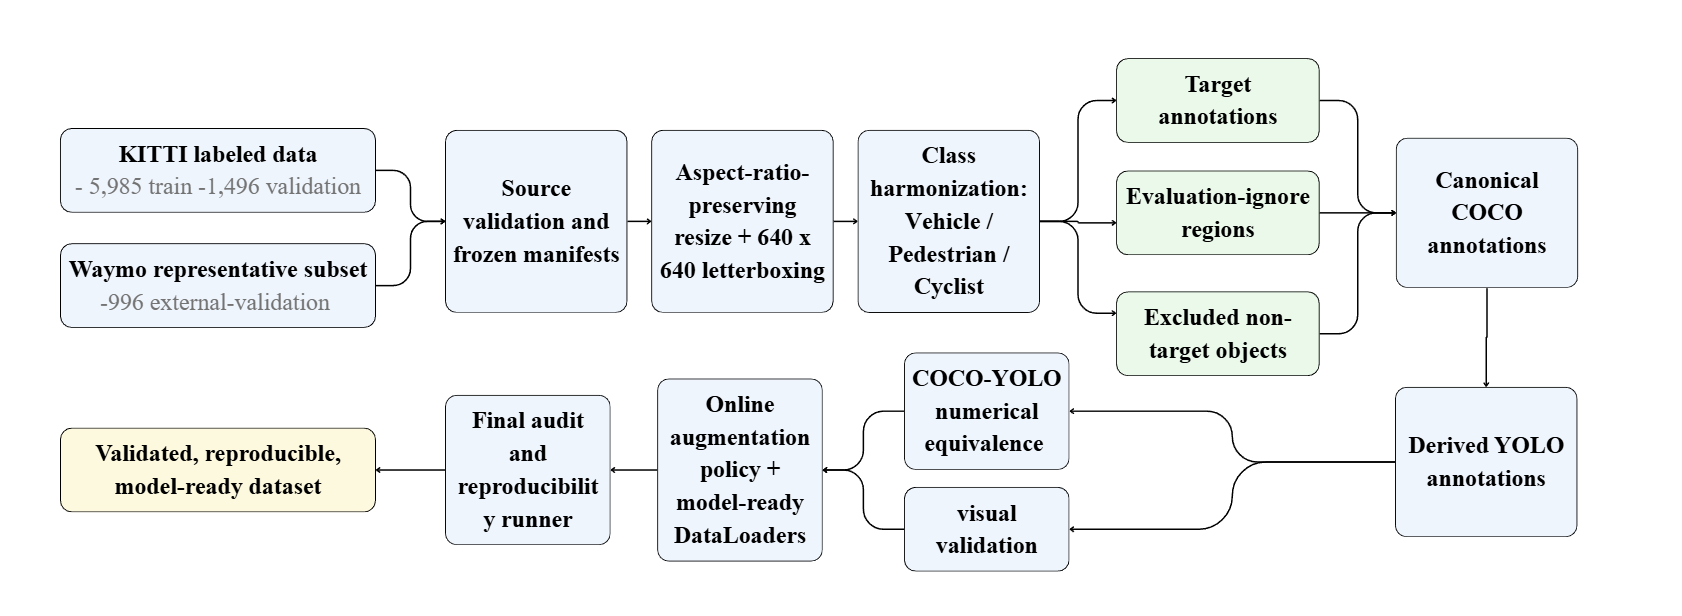
\includegraphics[width=\linewidth]{figures/pipeline.png}
    \caption{Unified preprocessing and validation pipeline. Frozen KITTI training and
    validation partitions and the Waymo external-validation subset are processed through
    common image standardization, class harmonization, annotation conversion, independent
    validation, controlled augmentation, model-ready loading, and a final reproducibility
    audit.}
    \label{fig:pipeline}
\end{figure}

\subsection{Experimental Roles and Leakage Prevention}
\label{sec:methodology_roles}

The experimental roles of the three partitions were fixed before model development. KITTI
train ($5{,}985$ images) is the only partition permitted to update model parameters. KITTI
validation ($1{,}496$ images) is reserved for in-domain validation, checkpoint comparison,
and model-development decisions. The representative Waymo subset ($996$ FRONT-camera
images from $25$ driving segments) is reserved exclusively for final cross-dataset
evaluation. Waymo data are not used for training, fine-tuning, early stopping,
hyperparameter optimization, threshold selection, checkpoint selection, or
augmentation-source sampling, preventing external-domain information from influencing the
learned parameters or the selection of the final model. The information-flow boundary is
illustrated in Figure~\ref{fig:partition_roles}.

\begin{figure}[t]
    \centering
    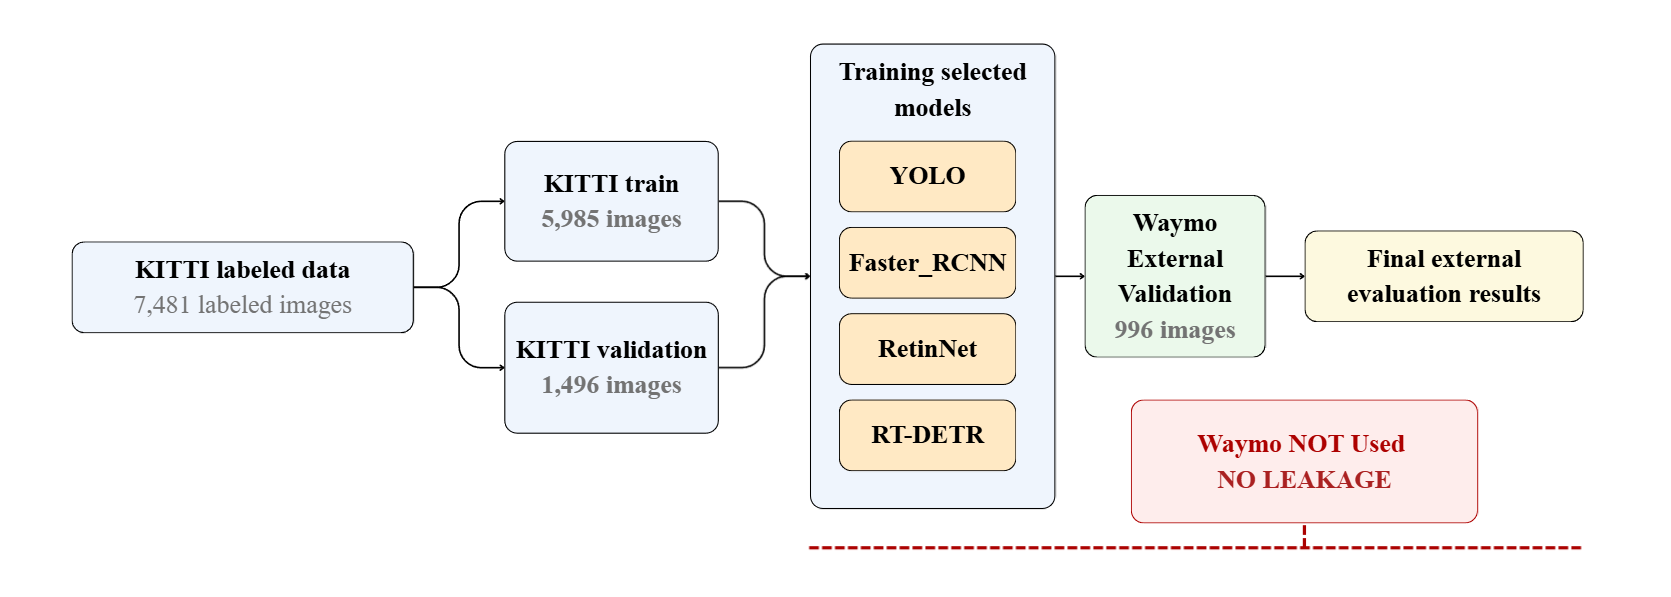
\includegraphics[width=\linewidth]{figures/partition_roles.png}
    \caption{Experimental partition roles and information-flow restrictions. KITTI train
    supports parameter learning, KITTI validation supports in-domain model development, and
    Waymo remains isolated until the final external evaluation of the selected model.}
    \label{fig:partition_roles}
\end{figure}

The Waymo subset preserves twelve images with no Vehicle, Pedestrian, or Cyclist
annotations; these target-negative scenes are retained intentionally because they support
later false-positive analysis under shifted driving conditions, and their empty labels are
treated as valid annotations rather than missing data.

\subsection{Image Standardization and Bounding-Box Transformation}
\label{sec:methodology_standardization}

The source datasets have substantially different image geometries: KITTI object-detection
images are typically wide road scenes close to $1{,}200\times370$ pixels, whereas the
selected Waymo FRONT-camera images have dimensions of $1{,}920\times1{,}280$ pixels.
Every source image was therefore converted to a common $640\times640$ representation using
aspect-ratio-preserving letterboxing. For an image of width $W$ and height $H$, the resize
factor was defined as $\min(640/W, 640/H)$; the resized image was centered within a
$640\times640$ canvas, and unused pixels were filled with the neutral gray value $114$ in
each channel. This procedure avoids geometric stretching while providing a fixed input
size for all detector families. The processed images were saved as PNG files to avoid
additional lossy compression.

Every bounding box was transformed using the exact scale and padding offsets applied to
its image, and transformed coordinates were checked against the processed-image boundary.
Across the complete set of $8{,}477$ images, preprocessing produced no missing outputs, no
invalid target boxes, no out-of-bound target boxes, and no clipped target boxes. Typical
KITTI images were resized to approximately $640\times193$ pixels with about $223$ pixels
of top padding and $224$ pixels of bottom padding, while Waymo images were resized to
approximately $640\times427$ pixels with about $106$ pixels of top and bottom padding.
Independent dry-run images confirmed that road content remained undistorted and that
transformed boxes remained attached to their source objects.

\subsection{Annotation Harmonization and Region Policy}
\label{sec:methodology_regions}

A common three-class taxonomy was frozen for the entire project. In the canonical COCO
representation these classes use identifiers $1$, $2$, and $3$, while in the derived YOLO
representation they use identifiers $0$, $1$, and $2$; the distinction preserves
compatibility with Torchvision, where class zero is reserved for background, and with
YOLO, where foreground classes begin at zero. The resulting combined target set contains
$49{,}678$ Vehicle boxes, $11{,}836$ Pedestrian boxes, and $2{,}391$ Cyclist boxes, for a
total of $63{,}905$ target annotations.

Target annotations were kept separate from two additional region types. KITTI DontCare
annotations were preserved as evaluation-ignore regions because eligible detections inside
these areas may be suppressed during evaluation instead of being counted as false
positives. KITTI Tram and Misc annotations were preserved as excluded non-target audit
regions; they are not project targets and do not automatically suppress false positives.
Waymo Sign and Unknown are assigned to the excluded category if encountered. The finalized
sidecars contain $11{,}295$ evaluation-ignore regions and $1{,}484$ excluded non-target
regions, none of which is inserted into the canonical COCO or derived YOLO target labels,
ensuring that training targets, evaluation suppression rules, and audit-only regions cannot
be confused by later model code.

\subsection{Canonical COCO and Derived YOLO Representations}
\label{sec:methodology_representations}

COCO was selected as the canonical target representation because it provides explicit image
and annotation identifiers, absolute pixel coordinates, named categories, and broad
framework compatibility. Three partition-specific files were created
(\texttt{kitti\_train.json}, \texttt{kitti\_val.json}, and
\texttt{waymo\_external.json}) with bounding boxes in the standard $[x, y, w, h]$
representation in absolute coordinates on the processed $640\times640$ images. The
canonical files contain $5{,}985$ KITTI training images with $31{,}294$ annotations,
$1{,}496$ KITTI validation images with $7{,}792$ annotations, and $996$ Waymo external
images with $24{,}819$ annotations (all $996$ Waymo records retained, including the twelve
with zero target annotations).

YOLO labels were derived from the canonical COCO files rather than generated independently
from the original sources. Each row stores the class identifier followed by normalized
center-$x$, center-$y$, width, and height values, serialized with ten decimal places, with
one label file per processed image (so the twelve target-negative Waymo images have valid
empty label files rather than absent labels). A framework adapter mirrors the validated
YOLO files beneath sibling images and labels directories expected by Ultralytics-style
pipelines; the adapter files are byte-identical to the canonical YOLO labels and do not
introduce a second ground-truth source.

\subsection{Numerical and Visual Validation}
\label{sec:methodology_validation}

A complete numerical equivalence test compared all $63{,}905$ canonical COCO boxes with
their serialized YOLO counterparts. Each YOLO box was reconstructed in processed-image
pixel coordinates and matched to the corresponding COCO box by image and class using
minimum-cost bipartite matching, so the result did not depend on annotation order. All
$63{,}905$ boxes were matched and classified as equivalent, with zero mismatched images;
the maximum normalized coordinate error was approximately $5.0\times10^{-11}$, the maximum
reconstructed pixel error approximately $4.8\times10^{-8}$ pixels, and the minimum
reconstructed intersection-over-union $0.9999998$. Visual comparisons for crowded,
cyclist-rich, pedestrian-rich, mixed, and target-negative scenes coincided between COCO
and YOLO overlays, with no boxes entering the gray letterbox padding.

\subsection{Augmentation Policy and Model-Ready Data Loading}
\label{sec:methodology_augmentation}

A conservative online augmentation policy was frozen for training. Augmentation is enabled
only for KITTI train and is disabled for KITTI validation and Waymo external evaluation;
no permanent augmented dataset is created. The permitted transformations are horizontal
flipping (probability $0.50$), brightness and contrast adjustment ($0.50$), HSV adjustment
($0.30$), and mild Gaussian blur ($0.10$). Vertical flipping, random cropping, arbitrary
rotation, perspective transformation, random scaling, shear, Mosaic, MixUp, Copy-Paste,
and Cutout are disabled, reducing unrealistic road geometry and preventing one detector
family from receiving framework-specific augmentation advantages. The random state is
derived from the base seed $42$, the training epoch, and the global image identifier,
making each augmented view reproducible.

A framework-neutral PyTorch dataset loader was implemented from the canonical COCO files,
returning a three-channel $640\times640$ float tensor, absolute XYXY boxes, canonical
labels, image and source identifiers, box areas, crowd flags, evaluation-ignore boxes,
excluded-object boxes, partition metadata, and an augmentation trace when training
augmentation is enabled, together with a detection-specific collation function supporting
variable numbers of objects per image. Smoke tests confirmed the expected partition
lengths, valid tensor and box shapes, finite values, correct class IDs, deterministic
validation behavior, valid target-negative handling, and a guard that prevents augmentation
from being enabled on validation or external partitions.

\subsection{Final Dataset Composition and Audit}
\label{sec:methodology_audit}

The final prepared dataset contains $8{,}477$ processed images and $63{,}905$ target
annotations, occupying approximately $2.1$~GiB. A read-only final audit combined the
outputs of all earlier validation stages with direct checks of physical images, COCO files,
canonical YOLO labels, framework labels, sidecar regions, manifests, issue files, and
visual artifacts, confirming exact class totals, valid empty labels for the twelve negative
images, zero partition overlap, complete COCO--YOLO equivalence, and correct DataLoader
behavior. The audit concluded with zero unresolved issues and a final status of PASSED.

% Experimental Setup
\section{Experimental Setup}
\label{sec:experimental_setup}

\subsection{Detectors}
\label{sec:setup_detectors}

Four representative detectors spanning the main detection paradigms were selected: YOLOv8s
(Ultralytics), a real-time one-stage CNN detector; RT-DETR-L (Ultralytics), a real-time
end-to-end transformer detector~\cite{zhao2024rtdetr}; RetinaNet (Torchvision), a dense
one-stage detector with focal loss~\cite{lin2017focalloss}; and Faster R-CNN (Torchvision),
a two-stage region-proposal detector~\cite{ren2015fasterrcnn}. All four operate on the
same three-class task and the same $640\times640$ letterboxed input, and all use
ImageNet-pretrained backbones.

\subsection{Training Protocol}
\label{sec:setup_training}

Training ran on Kaggle GPU notebooks (NVIDIA Tesla T4) across two compute slots, with
evaluation, benchmarking, and checkpoint locking performed locally. All models used an
effective batch size of $32$ (RT-DETR-L: $16$), a fixed random seed of $42$
(deterministic mode), an input size of $640\times640$, target epochs of $200$, and early
stopping with patience $20$ epochs on mAP@$[0.50{:}0.95]$. A $10.5$-hour runtime guard and
checkpoint/resume-state packaging supported interruption-expected runs; RT-DETR, RetinaNet,
and Faster R-CNN used validated multi-session resume chains. The online augmentation
policy described in Section~\ref{sec:methodology_augmentation} was applied to KITTI train
only.

\subsection{Evaluation Protocol}
\label{sec:setup_evaluation}

The primary evaluation metric is COCO Average Precision. mAP@$[0.50{:}0.95]$ is computed
over ten IoU thresholds from $0.50$ to $0.95$ in steps of $0.05$, together with AP50,
AP75, and per-class AP for Vehicle, Pedestrian, and Cyclist. Object size follows the COCO
definition: small ($<32^2$ px), medium ($32^2$--$96^2$ px), and large ($>96^2$ px).

In addition to the AP curve, a fixed operating point (confidence $\geq 0.25$, IoU $\geq
0.50$) is used to compute precision, recall, F1-score, detections per image, and false
positives per image. KITTI-specific ignore rules suppress a predicted box that overlaps a
DontCare region of the same class family by IoU $\geq 0.50$, so that it is neither counted
as a true positive nor as a false positive; Tram and Misc are excluded non-target classes.
Waymo has no DontCare-style ignore regions, and Sign boxes are excluded as a non-target
class.

For the Torchvision-based detectors (RetinaNet and Faster R-CNN), the training pipeline
applied ImageNet normalization through Albumentations in addition to the normalization
performed internally by the Torchvision detection models; evaluation therefore used the
same preprocessing configuration to avoid a train--evaluation distribution mismatch. The
Ultralytics-based YOLOv8s and RT-DETR models did not exhibit this issue. Confidence
thresholds and operating points were defined a priori and were not tuned using Waymo
results.

\subsection{External-Validation Methodology}
\label{sec:setup_external}

Waymo external validation reuses the frozen evaluation stack unchanged: predictions are
produced by the same adapters and metrics are computed with the same
\texttt{pycocotools} COCO evaluator, with only the dataset swapped from KITTI validation
($1{,}496$ images) to the Waymo external subset ($996$ images). The AP-curve confidence
threshold is $0.001$ (fixed before evaluation), and no threshold is tuned on Waymo.
Per-image inference time is measured during evaluation to produce the mean inference time
metric, while dummy-input latency, throughput, parameter count, and checkpoint size are
measured on the local GPU for the efficiency comparison.

% Results
\section{Results}
\label{sec:results}

\subsection{In-Domain Accuracy on KITTI}
\label{sec:results_kitti}

Table~\ref{tab:kitti_results} reports the KITTI in-domain results for the four detectors.
YOLOv8s achieves the highest accuracy on every axis, with mAP@$[0.50{:}0.95]$ of $0.690$,
AP50 of $0.925$, and AP75 of $0.780$. The accuracy ranking is YOLOv8s
($0.690$) $>$ RT-DETR-L ($0.606$) $>$ Faster R-CNN ($0.589$) $>$ RetinaNet ($0.537$).
Pedestrian is the weakest class across all four detectors ($0.392$--$0.530$), consistent
with the class's small object size and limited training instances, while Vehicle is the
strongest ($0.703$--$0.849$).

\begin{figure}[t]
    \centering
    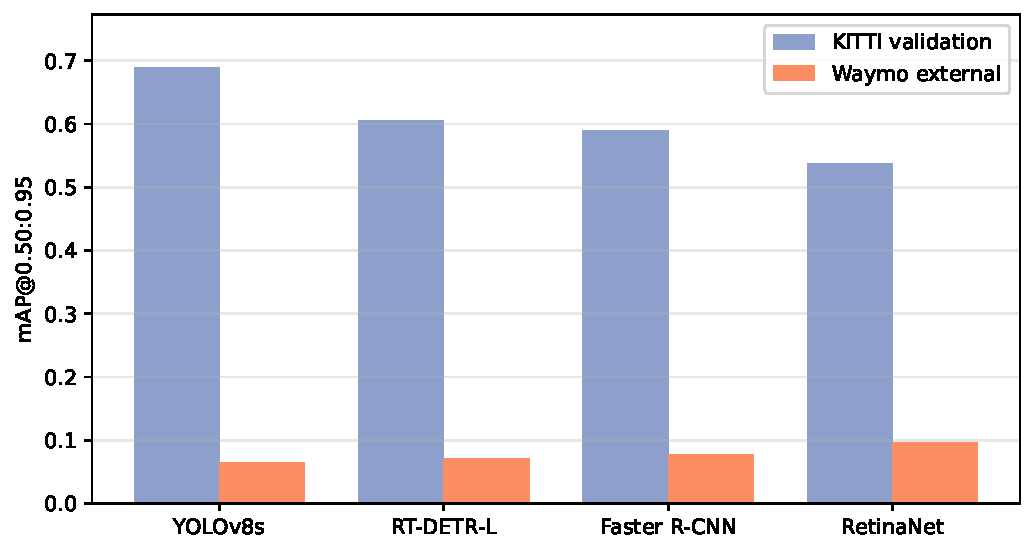
\includegraphics[width=\linewidth]{figures/kitti_vs_waymo_map50_95.pdf}
    \caption{KITTI in-domain versus Waymo external mAP@$[0.50{:}0.95]$ under target-free
    transfer. All detectors degrade sharply, and the in-domain ranking does not transfer to
    the external setting.}
    \label{fig:kitti_vs_waymo}
\end{figure}

\begin{table}[t]
    \centering
    \caption{KITTI in-domain detection results on the frozen validation split (1{,}496 images). Values are COCO Average Precision.}
    \label{tab:kitti_results}
    \begin{tabular}{lcccccc}
        \toprule
        Detector & mAP@0.50:0.95 & mAP@0.50 & mAP@0.75 & Vehicle AP & Pedestrian AP & Cyclist AP \\
        \midrule
        YOLOv8s & 0.690 & 0.925 & 0.780 & 0.849 & 0.530 & 0.691 \\
        RT-DETR-L & 0.606 & 0.906 & 0.679 & 0.730 & 0.490 & 0.597 \\
        Faster R-CNN & 0.589 & 0.879 & 0.666 & 0.741 & 0.432 & 0.594 \\
        RetinaNet & 0.537 & 0.839 & 0.577 & 0.703 & 0.392 & 0.518 \\
        \bottomrule
    \end{tabular}
\end{table}


\subsection{Computational Efficiency}
\label{sec:results_efficiency}

Table~\ref{tab:efficiency} summarizes the deployment-oriented efficiency comparison on the
local GPU. YOLOv8s is by far the most efficient detector: $11.1$M parameters, a $21.5$~MB
checkpoint, $12.36$~ms latency, and $94.77$~FPS. RT-DETR-L offers the second-best accuracy
but is considerably slower ($55.29$~ms, $18.73$~FPS). The two heaviest detectors carry a
large efficiency penalty: Faster R-CNN ($41.3$M parameters, $315.68$~MB, $91.22$~ms) and
RetinaNet ($36.4$M parameters, $278.0$~MB, $75.25$~ms).

\begin{table}[t]
    \centering
    \caption{Deployment-oriented efficiency comparison on the local GPU.}
    \label{tab:efficiency}
    \begin{tabular}{lcccc}
        \toprule
        Detector & Parameters (M) & Checkpoint (MB) & Latency (ms) & FPS \\
        \midrule
        YOLOv8s & 11.1 & 21.50 & 12.36 & 94.77 \\
        RT-DETR-L & 32.8 & 63.15 & 55.29 & 18.73 \\
        Faster R-CNN & 41.3 & 315.68 & 91.22 & 11.24 \\
        RetinaNet & 36.4 & 278.00 & 75.25 & 13.70 \\
        \bottomrule
    \end{tabular}
\end{table}


\subsection{Operating-Point Behavior}
\label{sec:results_operating_point}

At the fixed operating point (confidence $\geq 0.25$, IoU $\geq 0.50$,
Table~\ref{tab:operating_point}), YOLOv8s attains the highest precision ($0.926$) with a
high recall ($0.947$). RT-DETR-L emits many low-confidence detections (DETR-style
$300$ queries), so it achieves the highest recall ($0.969$) but the lowest precision
($0.482$) and the most false positives per image ($5.431$). Faster R-CNN and RetinaNet
fall between these two extremes.

\begin{table}[t]
    \centering
    \caption{Operating-point metrics on KITTI validation (confidence $\geq 0.25$, IoU $\geq 0.50$).}
    \label{tab:operating_point}
    \begin{tabular}{lcccc}
        \toprule
        Detector & Precision & Recall & F1 & FP/image \\
        \midrule
        YOLOv8s & 0.926 & 0.947 & 0.936 & 0.40 \\
        RT-DETR-L & 0.482 & 0.969 & 0.643 & 5.43 \\
        Faster R-CNN & 0.876 & 0.928 & 0.901 & 0.69 \\
        RetinaNet & 0.777 & 0.907 & 0.837 & 1.35 \\
        \bottomrule
    \end{tabular}
\end{table}


\subsection{Cross-Dataset External Validation on Waymo}
\label{sec:results_waymo}

Table~\ref{tab:waymo_results} reports the Waymo external-validation results obtained by
applying the four KITTI-trained checkpoints directly to the frozen Waymo subset with no
retraining. All detectors degrade sharply: mAP@$[0.50{:}0.95]$ falls to
$0.065$--$0.097$, an order of magnitude below the KITTI baseline
(Figure~\ref{fig:kitti_vs_waymo}). RetinaNet achieves the highest Waymo accuracy
($0.097$), followed by Faster R-CNN ($0.077$), RT-DETR-L ($0.071$), and YOLOv8s ($0.065$),
the reverse of the in-domain ranking.

\begin{table}[t]
    \centering
    \caption{Waymo external-validation results (996 front-camera images, no retraining).}
    \label{tab:waymo_results}
    \begin{tabular}{lcccccc}
        \toprule
        Detector & mAP@0.50 & mAP@0.50:0.95 & Vehicle AP & Pedestrian AP & Cyclist AP & Mean inf. (ms) \\
        \midrule
        YOLOv8s & 0.142 & 0.065 & 0.106 & 0.049 & 0.042 & 34.21 \\
        RT-DETR-L & 0.151 & 0.071 & 0.116 & 0.058 & 0.041 & 62.57 \\
        Faster R-CNN & 0.175 & 0.077 & 0.123 & 0.070 & 0.038 & 92.07 \\
        RetinaNet & 0.215 & 0.097 & 0.144 & 0.075 & 0.072 & 77.50 \\
        \bottomrule
    \end{tabular}
\end{table}


Table~\ref{tab:kitti_vs_waymo} quantifies the degradation and the generalization ratio
(Waymo mAP divided by KITTI mAP). Relative mAP@$[0.50{:}0.95]$ drops range from $82.0\%$
(RetinaNet) to $90.5\%$ (YOLOv8s), and generalization ratios range from $0.095$ (YOLOv8s)
to $0.180$ (RetinaNet), as shown in Figure~\ref{fig:generalization_ratio}. The best
generalizing detector is RetinaNet and the worst is YOLOv8s.

\begin{figure}[t]
    \centering
    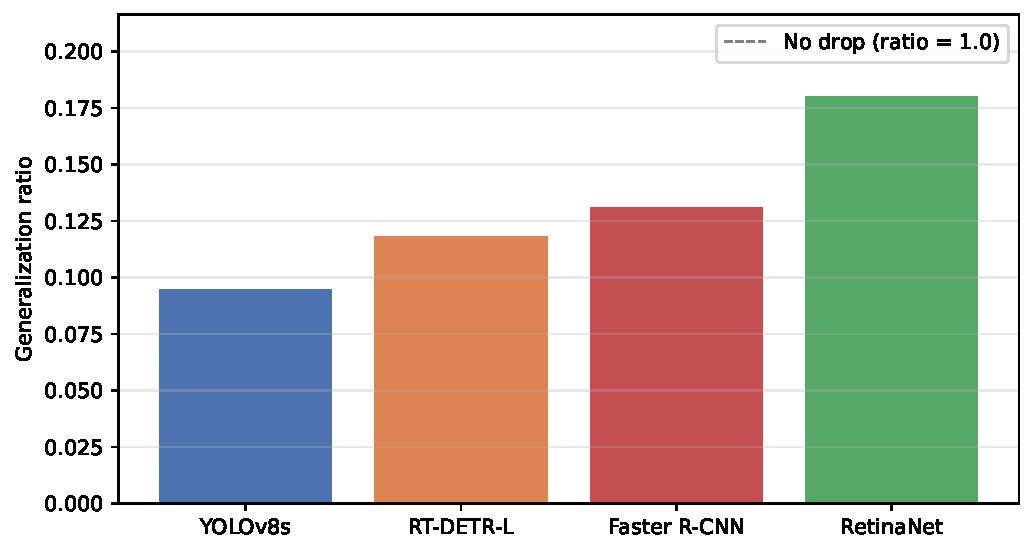
\includegraphics[width=\linewidth]{figures/generalization_ratio_map50_95.pdf}
    \caption{Generalization ratio (Waymo mAP@$[0.50{:}0.95]$ / KITTI mAP@$[0.50{:}0.95]$)
    for the four detectors. Higher values indicate greater cross-domain stability.}
    \label{fig:generalization_ratio}
\end{figure}

\begin{table}[t]
    \centering
    \caption{KITTI-to-Waymo degradation in mAP@0.50:0.95 and generalization ratio.}
    \label{tab:kitti_vs_waymo}
    \begin{tabular}{lccccc}
        \toprule
        Detector & KITTI mAP & Waymo mAP & Abs. drop & Drop (\%) & Gen. ratio \\
        \midrule
        YOLOv8s & 0.690 & 0.065 & 0.625 & 90.52 & 0.095 \\
        RT-DETR-L & 0.606 & 0.071 & 0.534 & 88.21 & 0.118 \\
        Faster R-CNN & 0.589 & 0.077 & 0.512 & 86.92 & 0.131 \\
        RetinaNet & 0.538 & 0.097 & 0.441 & 81.98 & 0.180 \\
        \bottomrule
    \end{tabular}
\end{table}


\subsection{Class-Wise Degradation}
\label{sec:results_class_wise}

Table~\ref{tab:class_wise_degradation} reports per-class AP@$[0.50{:}0.95]$ on both
datasets together with the absolute and relative drop. Vehicle exhibits the largest
absolute drop across detectors (Figure~\ref{fig:class_wise_degradation}), reflecting its
high in-domain score combined with a large distributional shift in scale and appearance on
Waymo. Cyclist shows the largest relative drop (up to $94.0\%$), while Pedestrian degrades
least in absolute terms but from a low baseline.

\begin{figure}[t]
    \centering
    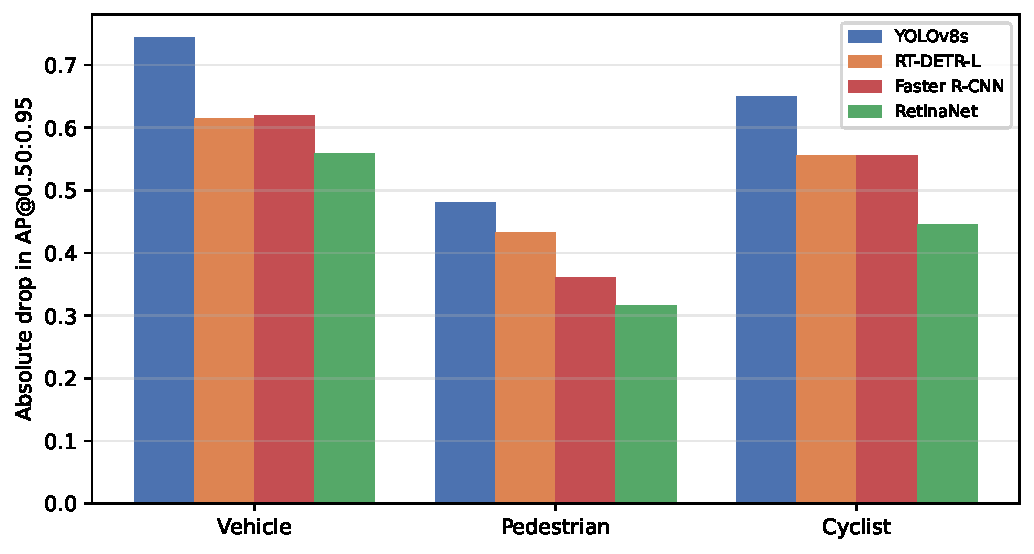
\includegraphics[width=\linewidth]{figures/class_wise_degradation.pdf}
    \caption{Class-wise absolute degradation in AP@$[0.50{:}0.95]$ (KITTI minus Waymo) by
    detector.}
    \label{fig:class_wise_degradation}
\end{figure}

\begin{table}[t]
    \centering
    \caption{Class-wise cross-dataset degradation in AP@0.50:0.95.}
    \label{tab:class_wise_degradation}
    \begin{tabular}{llcccc}
        \toprule
        Detector & Class & KITTI AP & Waymo AP & Abs. drop & Drop (\%) \\
        \midrule
        YOLOv8s & Vehicle & 0.849 & 0.106 & 0.743 & 87.56 \\
         & Pedestrian & 0.530 & 0.049 & 0.481 & 90.74 \\
         & Cyclist & 0.691 & 0.042 & 0.649 & 93.98 \\
        \addlinespace
        RT-DETR-L & Vehicle & 0.730 & 0.116 & 0.615 & 84.17 \\
         & Pedestrian & 0.490 & 0.058 & 0.432 & 88.20 \\
         & Cyclist & 0.597 & 0.041 & 0.556 & 93.15 \\
        \addlinespace
        Faster R-CNN & Vehicle & 0.741 & 0.123 & 0.619 & 83.46 \\
         & Pedestrian & 0.432 & 0.070 & 0.362 & 83.74 \\
         & Cyclist & 0.594 & 0.038 & 0.556 & 93.54 \\
        \addlinespace
        RetinaNet & Vehicle & 0.703 & 0.144 & 0.559 & 79.54 \\
         & Pedestrian & 0.391 & 0.075 & 0.317 & 80.93 \\
         & Cyclist & 0.518 & 0.072 & 0.446 & 86.08 \\
        \bottomrule
    \end{tabular}
\end{table}


\subsection{Robustness and Safety-Oriented Analysis}
\label{sec:results_safety}

\subsubsection{Object-Size Analysis}
\label{sec:results_size}

Recall and miss rate were computed per detector, dataset, and size category at the
operating point (Table~\ref{tab:object_size_recall}). On KITTI, recall declines with
object size but remains high for all detectors ($0.88$--$0.96$ small-object recall); on
Waymo, small-object recall collapses, reaching $0.045$--$0.132$ across detectors
(Figure~\ref{fig:object_size_recall}). This indicates that small objects are the dominant
failure mode under domain shift, consistent with Waymo containing many more small and
distant objects.

\begin{figure}[t]
    \centering
    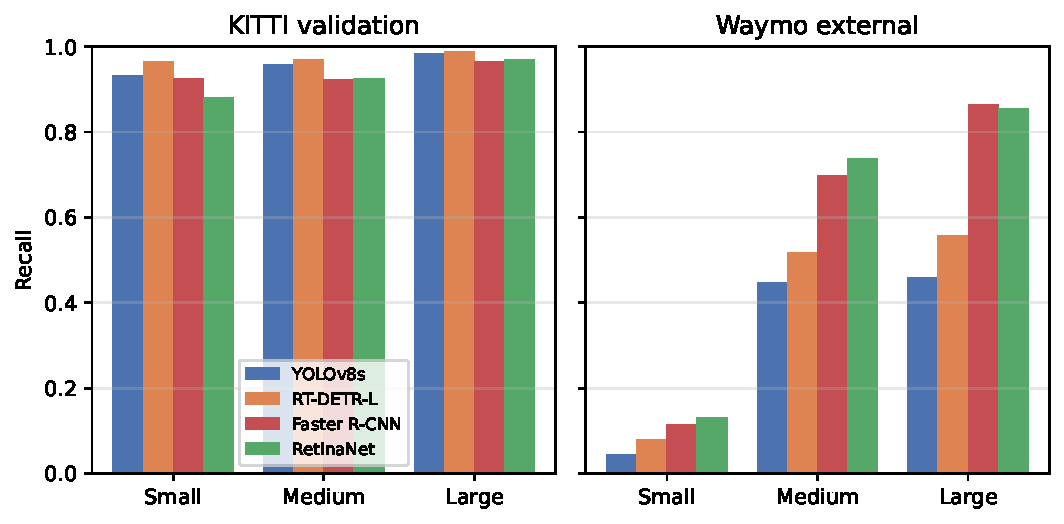
\includegraphics[width=\linewidth]{figures/object_size_recall.pdf}
    \caption{Recall by object-size category at the operating point for KITTI (left) and
    Waymo (right).}
    \label{fig:object_size_recall}
\end{figure}

\begin{table}[t]
    \centering
    \caption{Class-agnostic recall by object-size category at the frozen operating point (confidence $\geq 0.25$, IoU $\geq 0.50$).}
    \label{tab:object_size_recall}
    \begin{tabular}{lcccccc}
        \toprule
        Detector & \multicolumn{3}{c}{KITTI recall} & \multicolumn{3}{c}{Waymo recall} \\
        & Small & Medium & Large & Small & Medium & Large \\
        \midrule
        YOLOv8s & 0.932 & 0.958 & 0.985 & 0.045 & 0.448 & 0.460 \\
        RT-DETR-L & 0.964 & 0.971 & 0.989 & 0.081 & 0.517 & 0.558 \\
        Faster R-CNN & 0.925 & 0.923 & 0.966 & 0.115 & 0.697 & 0.865 \\
        RetinaNet & 0.881 & 0.926 & 0.970 & 0.132 & 0.737 & 0.855 \\
        \bottomrule
    \end{tabular}
\end{table}


\subsubsection{Safety-Critical False Negatives}
\label{sec:results_safety_fn}

False-negative rates for the safety-priority classes (Pedestrian and Cyclist) were computed
separately from overall accuracy (Table~\ref{tab:safety_fn}). On Waymo, the combined
pedestrian-plus-cyclist false-negative rate is $0.81$--$0.93$ for all detectors
(Figure~\ref{fig:pedestrian_cyclist_fn}), a safety-relevant result that is not visible
from average mAP alone: even the detector with the best Waymo mAP misses the large majority
of vulnerable road users.

\begin{figure}[t]
    \centering
    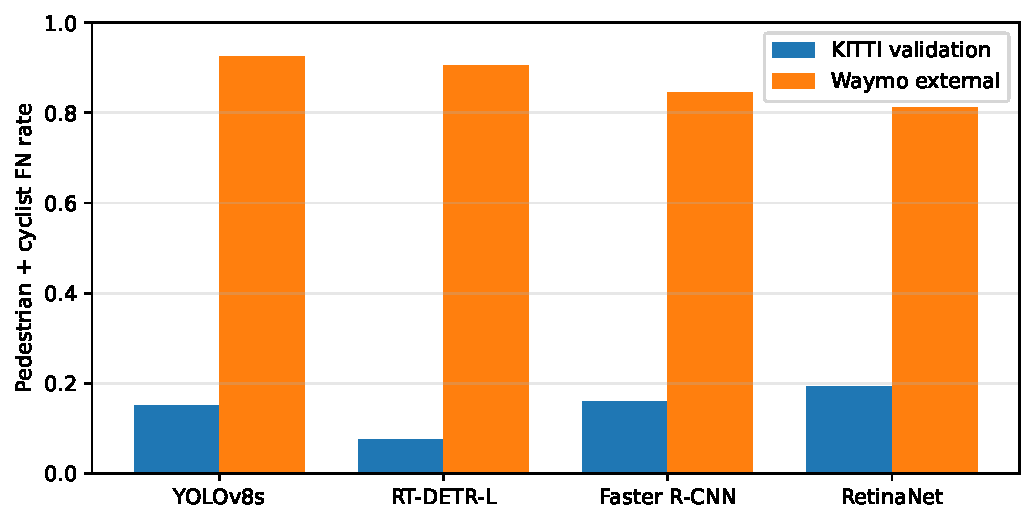
\includegraphics[width=\linewidth]{figures/pedestrian_cyclist_fn_rate.pdf}
    \caption{Safety-critical false-negative rate for pedestrians and cyclists at the
    operating point, for KITTI and Waymo.}
    \label{fig:pedestrian_cyclist_fn}
\end{figure}

\begin{table}[t]
    \centering
    \caption{Safety-critical false-negative rate for pedestrians and cyclists (operating point, confidence $\geq 0.25$, IoU $\geq 0.50$).}
    \label{tab:safety_fn}
    \begin{tabular}{lcc}
        \toprule
        Detector & KITTI FN rate & Waymo FN rate \\
        \midrule
        YOLOv8s & 0.152 & 0.926 \\
        RT-DETR-L & 0.077 & 0.906 \\
        Faster R-CNN & 0.159 & 0.844 \\
        RetinaNet & 0.194 & 0.811 \\
        \bottomrule
    \end{tabular}
\end{table}


\subsubsection{Failure-Type Decomposition}
\label{sec:results_failure_type}

Table~\ref{tab:failure_type} decomposes detections into true positives, missed detections,
false positives, localization errors, class confusions, and over-detections. On KITTI,
RT-DETR-L emits the most false positives and by far the most over-detections, consistent
with its low operating-point precision. On Waymo, missed detections dominate for every
detector, again reflecting the collapse of small-object recall.

\begin{table}[t]
    \centering
    \caption{Failure-type decomposition at the operating point for KITTI and Waymo.}
    \label{tab:failure_type}
    \begin{tabular}{llcccccc}
        \toprule
        Dataset & Detector & TP & Miss (FN) & FP & Localization & Confusion & Over-detect. \\
        \midrule
        KITTI & YOLOv8s & 7,382 & 410 & 163 & 272 & 15 & 142 \\
         & RT-DETR-L & 7,551 & 241 & 777 & 1,620 & 82 & 5,646 \\
         & Faster R-CNN & 7,231 & 561 & 241 & 592 & 96 & 98 \\
         & RetinaNet & 7,069 & 723 & 425 & 1,165 & 161 & 274 \\
        \addlinespace
        Waymo & YOLOv8s & 2,721 & 22,098 & 20 & 132 & 56 & 27 \\
         & RT-DETR-L & 3,769 & 21,050 & 40 & 446 & 132 & 743 \\
         & Faster R-CNN & 5,269 & 19,550 & 292 & 1,263 & 366 & 78 \\
         & RetinaNet & 5,771 & 19,048 & 328 & 2,007 & 561 & 216 \\
        \bottomrule
    \end{tabular}
\end{table}


\subsection{Deployment Trade-Off}
\label{sec:results_deployment}

Table~\ref{tab:deployment} and Figure~\ref{fig:deployment_tradeoff} jointly summarize
in-domain accuracy, external accuracy, latency, and vulnerable-road-user (VRU) safety on
Waymo (the VRU false-negative rate and the small-object recall restricted to pedestrians
and cyclists). No single detector simultaneously optimizes accuracy, generalization,
latency, and safety: YOLOv8s is fastest and most accurate in-domain but least stable and
safety-reliable out-of-domain, while RetinaNet generalizes best and is most safety-reliable
on Waymo but is slower and weaker in-domain.

\begin{figure}[t]
    \centering
    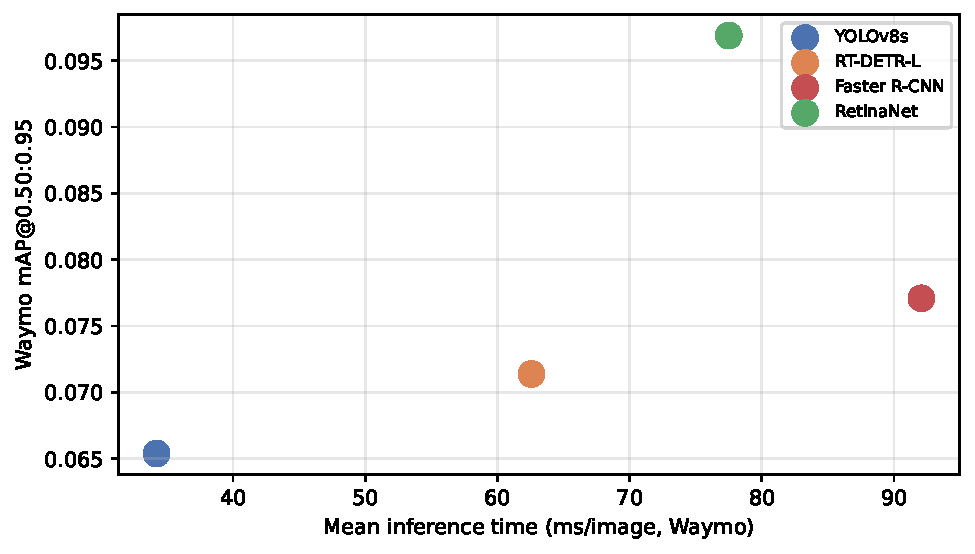
\includegraphics[width=\linewidth]{figures/deployment_tradeoff.pdf}
    \caption{Deployment trade-off between mean inference time and Waymo mAP@$[0.50{:}0.95]$.}
    \label{fig:deployment_tradeoff}
\end{figure}

\begin{table}[t]
    \centering
    \caption{Deployment trade-off: in-domain accuracy, external accuracy, latency, and vulnerable-road-user (VRU) safety on Waymo.}
    \label{tab:deployment}
    \begin{tabular}{lccccc}
        \toprule
        Detector & KITTI mAP & Waymo mAP & Latency (ms) & Waymo VRU FN & Waymo VRU small recall \\
        \midrule
        YOLOv8s & 0.690 & 0.065 & 34.21 & 0.926 & 0.029 \\
        RT-DETR-L & 0.606 & 0.071 & 62.57 & 0.906 & 0.047 \\
        Faster R-CNN & 0.589 & 0.077 & 92.07 & 0.844 & 0.097 \\
        RetinaNet & 0.537 & 0.097 & 77.50 & 0.811 & 0.127 \\
        \bottomrule
    \end{tabular}
\end{table}


% Discussion
\section{Discussion}
\label{sec:discussion}

\subsection{Domain Shift and Ranking Inversion}
\label{sec:discussion_shift}

All four detectors experience a severe accuracy drop when transferred from KITTI to Waymo,
with mAP@$[0.50{:}0.95]$ falling by roughly $80$--$90\%$ relative to the in-domain
baseline. This is expected for a direct, no-retraining cross-dataset transfer: KITTI and
Waymo differ in camera calibration, sensor position, scene composition, object-scale
distribution, and annotation density. More consequential is the inversion of the detector
ranking across domains. YOLOv8s, the strongest in-domain detector, shows the lowest
generalization ratio ($0.095$), while RetinaNet, the weakest in-domain detector, generalizes
best ($0.180$). This inversion is a candidate indicator of overfitting to KITTI-specific
statistics for the higher-capacity detectors, and it demonstrates that the in-domain
ranking does not transfer to the out-of-domain setting.

The pattern is consistent with the architecture families. The real-time CNN and transformer
detectors (YOLOv8s and RT-DETR) achieve the highest in-domain accuracy but the strongest
relative degradation, whereas the two Torchvision detectors trained with a conservative,
fixed augmentation policy degrade less in relative terms. This does not establish a causal
mechanism, but it suggests that the choice of training regime and architecture interacts
with domain shift in a way that in-domain validation alone cannot reveal.

\subsection{Small Objects and Vulnerable Road Users}
\label{sec:discussion_safety}

The safety-oriented analysis shows that the dominant failure mode is missed detection of
small objects, and that this is far more severe on Waymo than on KITTI. On KITTI,
small-object recall is $0.88$--$0.96$ across detectors, whereas on Waymo it is
$0.03$--$0.13$. Consequently, the pedestrian-plus-cyclist false-negative rate on Waymo
reaches $0.81$--$0.93$ for all detectors. This result is invisible in average mAP: the
detector with the highest Waymo mAP is not the most safety-reliable, because average
precision is dominated by large, easily detected vehicles. For intelligent-vehicle
perception, small-object and pedestrian/cyclist recall should therefore be treated as
first-class deployment metrics alongside mAP, and safety-critical evaluation should be
reported at a fixed operating point rather than only as an AP curve.

\subsection{Deployment Implications}
\label{sec:discussion_deployment}

The efficiency results reinforce the need for a joint accuracy--efficiency--safety
assessment. YOLOv8s provides an order-of-magnitude latency advantage and the best in-domain
accuracy but the least external stability and safety reliability, making it attractive only
when latency is the binding constraint and in-domain statistics match deployment. RetinaNet
offers the best external generalization and safety-oriented recall but at substantially
higher latency and model size, making it attractive when out-of-domain reliability is
prioritized over speed. RT-DETR-L suffers from a large number of low-confidence
over-detections at the fixed operating point, and Faster R-CNN is the slowest detector
despite mid-range accuracy. The practical implication is that detector selection must be
based on external validation and safety metrics rather than KITTI mAP alone, and that the
choice depends on the deployment priority: latency, in-domain accuracy, or out-of-domain
safety.

\subsection{Interpretation and Limitations of the Comparison}
\label{sec:discussion_interpretation}

These findings are descriptive and correlational: the study quantifies how, where, and why
the four detectors fail under a controlled target-free transfer, but it does not isolate
the causal contribution of architecture, capacity, or training regime. The relative
stability of RetinaNet, for instance, could reflect its conservative training setup as much
as its architecture. Nevertheless, the results provide a reproducible evidence base for
deployment-oriented perception and a concrete motivation for domain-robust training or
adaptation strategies~\cite{chen2018domainadaptive,li2022crossdomainadaptive}, which the
target-free setting deliberately leaves out.

% Threats to Validity
\section{Threats to Validity}
\label{sec:threats}

Several limitations bound the interpretation of these results.

\textbf{Subset size and coverage.} The Waymo external subset ($996$ images) is smaller than
the KITTI validation split ($1{,}496$ images) and represents a single camera view (FRONT)
sampled every fifth frame from $25$ segments. The subset was selected to maximize coverage
of rare conditions (night, dawn/dusk, the single rainy segment), but it cannot represent
the full diversity of the Waymo dataset, and conclusions should not be generalized beyond
this configuration.

\textbf{Operating point.} The robustness and safety analyses are confined to the frozen
operating point (confidence $0.25$, IoU $0.50$); results may differ at other operating
points, and no threshold is tuned on Waymo, so operating-point precision/recall reflect the
a priori threshold rather than an optimized one.

\textbf{Inference-time comparability.} Waymo inference time is measured per real image
including first-image warmup, and is not directly comparable to the dummy-input benchmark
latency reported in the efficiency comparison; the two measures serve different purposes.

\textbf{Failure-type classification.} The failure-type decomposition uses documented
IoU-based heuristics, and ambiguous cases are resolved by a fixed priority order. The
classification is therefore descriptive rather than definitive, and counts of localization
errors, confusions, and over-detections should be interpreted relative to each other rather
than as absolute error frequencies.

\textbf{Preprocessing note.} The Torchvision-based detectors applied training-time ImageNet
normalization through Albumentations in addition to the normalization performed internally
by the detection models, and evaluation used the same configuration. This avoids a
train--evaluation mismatch but means the exact preprocessing path differs across
frameworks, a practical characteristic of a cross-family comparison.

\textbf{Scope.} Results are specific to the locked checkpoints, the frozen split, the
three-class task, and the evaluated hardware. The study makes no causal claims and does not
claim state-of-the-art performance or a novel architecture; the contribution is a
reproducible external-validation methodology and evidence base.

% Conclusion
\section{Conclusion}
\label{sec:conclusion}

This study presented a controlled target-free cross-dataset evaluation of four detector
families---YOLOv8s, Faster R-CNN, RetinaNet, and RT-DETR---trained on KITTI and externally
validated on a representative Waymo front-camera subset. The evaluation unified in-domain
accuracy, absolute and relative cross-dataset degradation, a generalization ratio,
class-wise behavior, safety-oriented failure analysis, and same-hardware efficiency under a
harmonized three-class protocol.

The results show that strong in-domain accuracy does not translate into robust external
performance. All detectors degrade sharply under target-free transfer, with
mAP@$[0.50{:}0.95]$ falling from $0.538$--$0.690$ on KITTI to $0.065$--$0.097$ on Waymo
and generalization ratios of $0.095$--$0.180$. The in-domain ranking inverts: YOLOv8s is
strongest in-domain yet least stable, while RetinaNet is weakest in-domain yet most stable
out-of-domain. Safety-oriented analysis further shows that small objects and vulnerable
road users dominate the failures, with pedestrian-plus-cyclist false-negative rates of
$0.81$--$0.93$ on Waymo even for the most accurate detector. No single detector
simultaneously optimizes accuracy, generalization, latency, and safety.

These findings indicate that detector selection for intelligent-vehicle perception should
be based on external validation and safety metrics rather than in-domain mAP alone, and
they motivate domain-robust training or adaptation strategies as a natural next step. By
preserving a reproducible pipeline from raw results to paper tables and figures, the study
also provides an evidence base that can be regenerated as the underlying datasets, models,
or evaluation protocol evolve.


\bibliographystyle{unsrt}
\bibliography{references}

\end{document}
